\chapter{The QDOAS Tools} \label{cha:tools}
QDOAS is delivered with four off-line modules :

\begin{itemize} \itemsep -6pt
\item \textbf{convolution} : a convolution/filtering tool;
\item \textbf{Ring} : a tool to create Ring effect cross sections;
\item \textbf{usamp} : a tool to create undersampling cross sections;
\item \textbf{doas\_cl} : a command line tool for batch processing.
\end{itemize}

The three first ones were already in WinDOAS. If they can still be called from
the QDOAS user interface, they are separate executables with their own user
interface, menu options and XML configuration files.

\section{The convolution/filtering tool (convolution)}\label{sec:conv-tool}

The \textbf{Convolution/Filtering} tool gives the possibility :

\begin{itemize}
\item to convolve spectra and cross sections;

\begin{itemize} \itemsep -6pt
\item user-defined slit functions and analytical line shapes are accepted;
\item convolution with $I_0$ correction is supported;
\end{itemize}

\item to shift the calibration grid before convolution;
\item to create an effective slit function taking into account the (finite) resolution
of the source spectrum (using a FT deconvolution method);
\item to apply a low-pass or a high-pass filter to the convolved cross section
before saving it.
\end{itemize}

\textbf{Convolution/Filtering} tool options are distributed in three pages :
\vskip 6pt
\begin{tabular}[h]{l p{8cm}}
\textbf{General} & general options (convolution type, input/output files...); \\ [6pt]
\textbf{Slit} & selection and parameterisation of the slit function; \\ [6pt]
\textbf{Filtering} & selection and parameterisation of the filter; \\ [6pt]
\end{tabular}

\begin{figure}[!h]
\subsection{The General Page}\hfill
\vspace{-.8\baselineskip}
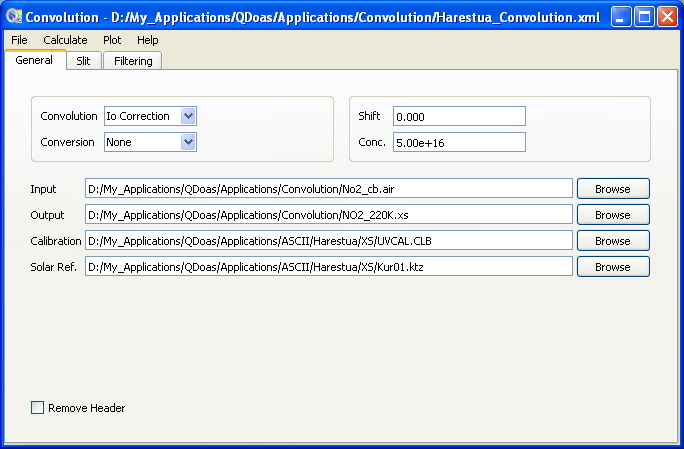
\includegraphics[width=1\textwidth]{img/Tools_Convolution_General.jpg}
\caption{Convolution/Filtering Tool} \label{tools_convolution_general}
\end{figure}
\FloatBarrier

\subsubsection{The Convolution Type}

QDOAS supports standard convolution and convolution with $I_0$ correction. The
convolution integral is calculated using the method of trapezes. If \textbf{None} is
selected, the cross section is just interpolated on the final grid.

\subsubsection{Conversion}

Before the convolution, it is possible to convert the original wavelength
calibration of the input cross section file from the air to the vacuum or inversely,
from the vacuum to the air.

\subsubsection{Requested Files Names}\hfill
\begin{tabular}[t]{l p{9.5 cm}}
\textbf{Input file} & the name of the high resolution cross section file to interpolate or convolve;   \\ [6pt]
\textbf{Output file} & the name of the resulting interpolated or convolved cross section file;  \\ [6pt]
\textbf{Calibration} & the final grid on which the original cross section (input file) must be interpolated or convolved;  \\ [6pt]
\textbf{Solar ref.} & the high-resolution solar spectrum requested only if the convolution with $I_0$ correction is selected;  \\ [6pt]
\end{tabular}

The format of input and output files is described in appendices \textbf{\ref{cha:input-files-format}} and \textbf{\ref{cha:output}}. The resulting cross section
file can be used as input for the retrieval. It is then better to give the
name of the output file in the format imposed by QDOAS : \textbf{cross section
files names must imperatively start with the symbol name as prefix
followed by the underscore character!}

\subsubsection{Shifting the Convolved cross section}

A shift in nm can be applied to the convolved cross section. In order to avoid
interpolation after convolution, this shift is applied on the calibration grid before
convolution.

\subsubsection{$I_0$ correction}

The fields \textbf{Solar Ref.} and \textbf{Conc} are respectively the name of the high resolution
solar spectrum file and the scaling column density of the concerned molecule.
Both are used for calculating the synthetic optical density in the formula of $I_0$
correction convolution. These fields are ignored if $I_0$ correction is not used.

\begin{figure}[!h]
\subsection{The Slit Function Page}\label{sec:slit-function-page}\hfill
\vspace{-.8\baselineskip}
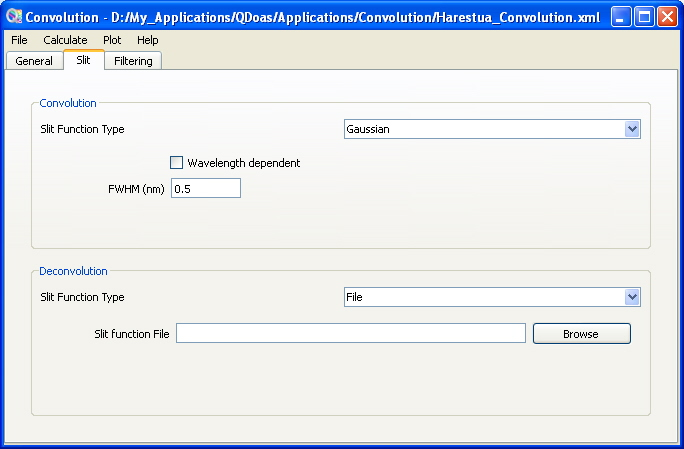
\includegraphics[width=1\textwidth]{img/Tools_Convolution_Slit.jpg}
\caption{Convolution/Filtering Tool: Slit Function page} \label{tools_convolution_slit}
\end{figure}
\FloatBarrier

This page is dedicated to the selection and the parameterisation of the convolution slit function.  Different analytical line shapes (Gaussian, Lorentzian, Voigt, error functions, asymmetric gaussian) are supported.  \textbf{QDOAS always requests the FWHM of the line shapes}.  The wavelength dependency of the slit function parameters characterized by the wavelength calibration procedure can be saved from the plot page in order to be accounted for the convolution.  Check the \textbf{Wavelength dependent} button to enter files instead of numbers.  Refer to the section \textbf{\nameref{sec:analyt-line-shap}} on page \pageref{sec:analyt-line-shap}, for further information on the supported analytical line shapes.

The use of arbitrary slit functions is possible with \textbf{File} option.  Look up table of slit functions defined at specific wavelengths is accepted.  If the \textbf{Wavelength dependent} button is checked, a three columns file is expected giving the variation of two different stretch factors to apply on the grid of the slit function.  Such a file can be obtained by merging in one file the SFP1 and SFP2 parameters resulting from the wavelength calibration procedure.

See file formats in \textbf{\nameref{cha:input-files-format} Annex}.


\subsubsection{Deconvolution}

A deconvolution slit function can also be defined.  In this case, the high resolution cross section is convolved using an effective slit function obtained from the FT of convolution and deconvolution slit functions.  This feature doesn’t work if a wavelength dependent slit function is selected.  By default, no deconvolution is applied.

\begin{figure}[!ht]
\subsection{The Filtering Page}\hfill
\vspace{-.8\baselineskip}
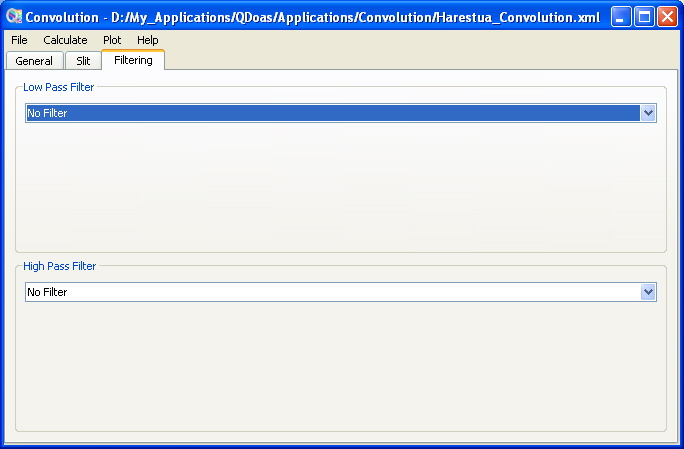
\includegraphics[width=1\textwidth]{img/Tools_Convolution_Filtering.jpg}
\caption{Convolution/Filtering Tool: Filtering page}
\label{tools_convolution_filtering}
\end{figure}
\FloatBarrier

After convolution, a low-pass and/or a high-pass filtering can be applied on the cross section.  By default, no filtering is applied.  The presentation of this page is the same as the \textbf{Filtering} one of \textbf{Projects properties}.  According to the selected filter type, the requested information can be different.

The original spectrum can be divided by the smoothed one or the smoothed spectrum can be subtracted from the original one.  The second feature is useful to create differential cross sections.

\subsubsection{The Convolution}

Once the parameters specified, the convolution is performed using the \textbf{Calculate $\rightarrow$ Run Convolution} option from the menu bar.   The original cross section and the convolved one (respectively in black and in red on the plot below) are displayed.  In order to avoid edge effects, the convolution has been performed on a larger interval but only the part of the convolved spectrum defined on the final grid is output.  If a filtering has been applied, another plot follows, with the original cross section and the resulting one after convolution and filtering.

\begin{figure}[!h]
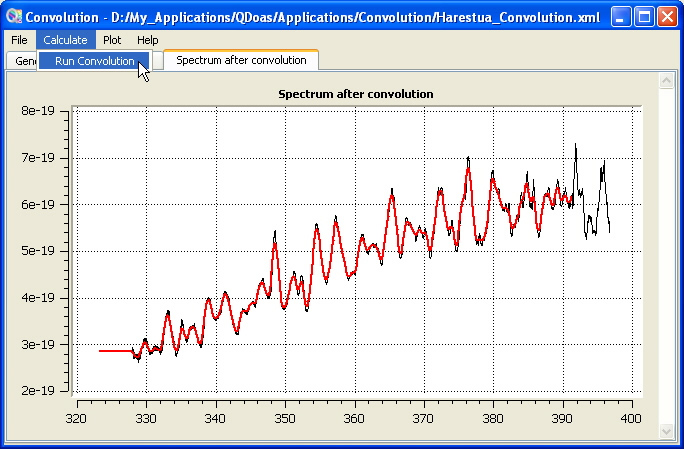
\includegraphics[width=1\textwidth]{img/Tools_Convolution.jpg}
\caption{Convolution with $I_0$ correction of a \NO2 cross section
  with a Gaussian (FWHM : 0.5 nm)
  \citep{vandaele1996}} \label{tools_convolution}
\end{figure}
\FloatBarrier

\section{The Ring tool (ring)}

The so-called Ring effect arises in the atmosphere due to inelastic scattering processes (mainly \gls{rrs} by molecular \oxygen{} and \N2). Roughly speaking, it manifests itself by a broadening of the solar and atmospheric spectral features present in measured spectra. This broadening typically reduces the depth of thin solar and atmospheric absorption features by several percents. Hence, it has a strong impact on spectroscopic measurements using the \gls{doas} method and retrieval algorithms must appropriately correct for it. This is especially true for minor absorbers like BrO or OClO, for which weak absorption features can be completely masked by Ring structures.

In DOAS, the Ring effect is usually accounted for as an absorber. The QDOAS Ring tool calculates Ring cross sections using a simple method described by \citet{Chance1997}.  See the \textbf{Description of Algorithms} chapter, page \pageref{sec:ring-effect} for further information on the Ring effect.

\begin{figure}[!h]
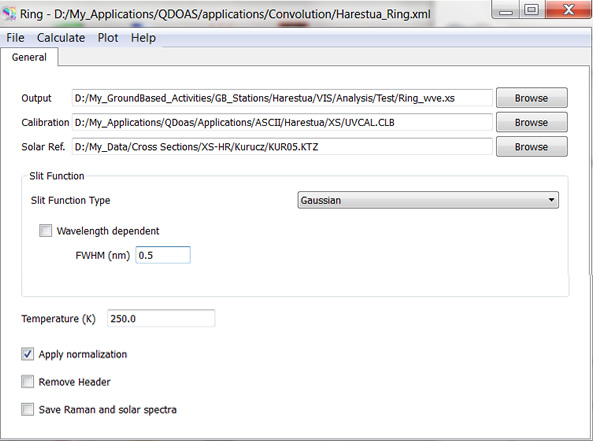
\includegraphics[width=1\textwidth]{img/Tools_Ring_General.jpg}
\caption{The Ring Tool}\label{tools_ring_general}
\end{figure}
\FloatBarrier

\subsubsection{Input}

QDOAS requires :

\begin{minipage}[t]{\textwidth}
\vspace{-1\baselineskip}
\begin{enumerate} \itemsep -6pt
\item the final grid on which the Ring cross section must be calculated;
\item a high-resolution solar spectrum;
\item the slit function to use for the convolution : user-defined slit functions and analytical line shapes (Gaussian, Lorentzian, Voigt and error functions) are accepted. The wavelength dependency of the line shape (Gaussian or error function) characterized by the wavelength calibration procedure can be saved from the plot page in order to be accounted for the convolution.
\end{enumerate}
\end{minipage}
\vskip 6pt
The effect of a change in temperature is small. Generally 250K is a good approximation for the atmospheric temperature at which most of the RRS is taking place.  The normalization of the Raman spectrum (see~\citep{Wagner2009}) is now optional

\subsubsection{Output}

As the calculated Ring cross section is accounted as an absorber, it is recommended to give the name of the output file in the format imposed by QDOAS : \textbf{cross section files names must imperatively start with the symbol name as prefix followed by the underscore characters!}

The Ring cross section is calculated as the ratio of the rotational
Raman spectrum by the solar spectrum (R/S).  The output file is an
ASCII file with two or four columns depending on whether the button ``Save
Raman and solar spectrum'' is checked or not: \vskip 3pt
\begin{minipage}[t]{\textwidth}
\vspace{-1\baselineskip}
\begin{itemize} \itemsep -6pt
\item the input wavelength calibration;
\item the calculated Ring cross section;
\item the interpolated Raman spectrum (optional);
\item the convolved solar spectrum (optional).
\end{itemize}
\end{minipage}
\vskip 6pt
To directly use the file as a cross section for the analysis without further convolution, only the first two columns should be saved (the program will display an error if the file contains unneeded columns).  If the \textbf{Convolve Ring} action is requested (see the \textbf{Molecules page} of \textbf{Analysis windows properties}), the program needs all four columns.  With ``Convolve Ring'', QDOAS uses the information on the slit function retrieved from the wavelength calibration procedure or from the slit function page to convolve the Raman and the solar spectra separately, and use the calculated ratio as a Ring cross section in the fit.

\begin{figure}[!h]
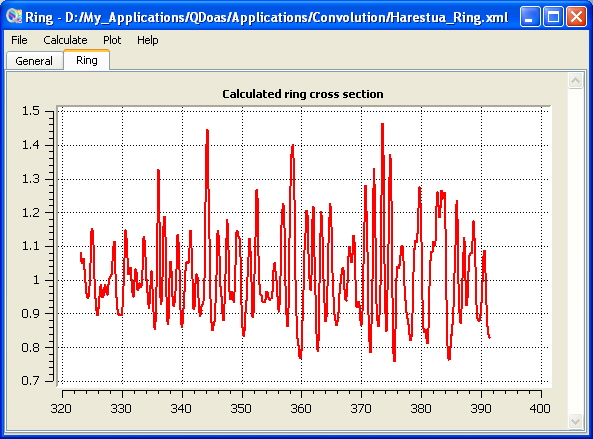
\includegraphics[width=1\textwidth]{img/Tools_Ring.jpg}
\caption{Ring cross section generated with the Ring Tool} \label{tools_ring}
\end{figure}
\FloatBarrier

\section{The undersampling tool (usamp)}  \label{sec:tool_undersampling}

The undersampling is a well-known problem of GOME onboard the satellite ERS-2. It arises from the poor sampling ratio of the GOME instrument (2 to 3 pixels/\gls{fwhm} of the resolution of the spectrometer) which results in a lost of spectral information when interpolating earthshine spectra during the DOAS fitting process. The problem can be corrected using ad-hoc cross sections obtained by simulating the effect from a high-resolution solar reference (see Chance K., 1998 \citep{Chance1998}).

The approach consists in building two spectra (an oversampled one and an undersampled one) from the high resolution solar spectrum and according to the selected analysis method, to calculate the ratio (DOAS fitting) or the difference (Intensity fitting) in order to simulate the interpolation error. Two undersampling cross sections are generated (the first one using the instrument grid and the second one using the instrument grid with a small shift applied).

See the \textbf{Description of Algorithms} chapter, page \pageref{sec:unders-corr}, for further information on the undersampling.

\begin{figure}[!h]
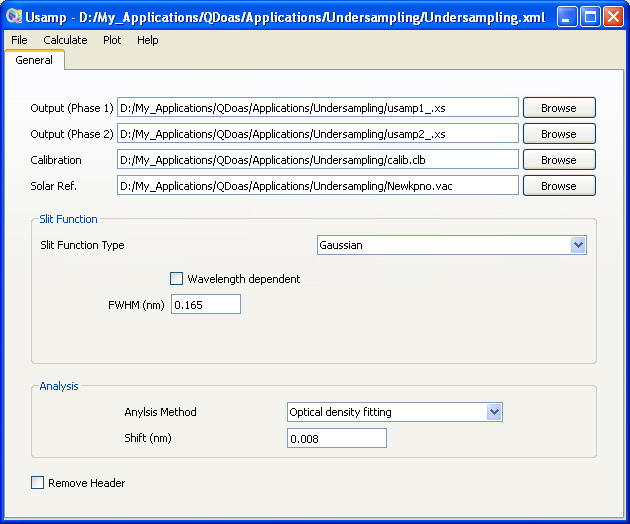
\includegraphics[width=1\textwidth]{img/Tools_Usamp_General.jpg}
\caption{The Undersampling Tool} \label{tools_usamp_general}
\end{figure}
\FloatBarrier

\subsubsection{Input}

QDOAS requires :

\begin{itemize}
\item the final grid on which the undersampling cross sections must be calculated;
\item a high-resolution solar spectrum;
\item the slit function to use for the convolution : user-defined slit functions and analytical line shapes (Gaussian, Lorentzian, Voigt and error functions) are accepted. The wavelength dependency of the line shape (Gaussian or error function) characterized by the wavelength calibration procedure can be saved from the plot page in order to be accounted for the convolution.
\item the shift to apply to oversampled and undersampled spectra in the calculation of undersampling;
\item the analysis method that determines the relation between oversampled and undersampled spectra;
\end{itemize}

\subsubsection{Output}

Two undersampling cross sections are generated by the procedure. It is recommended to give the name of the output files in the format imposed by QDOAS : \textbf{cross section files names must imperatively start with the symbol name as prefix followed by the underscore character~!}

\begin{figure}[!h]
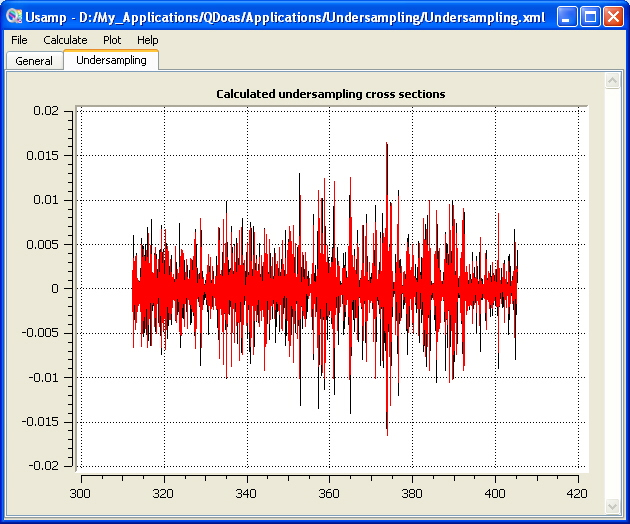
\includegraphics[width=1\textwidth]{img/Tools_Usamp_Plot.jpg}
\caption{Undersampling cross sections generated with the Undersampling Tool} \label{tools_usamp}
\end{figure}
\FloatBarrier

\section{The command line tool (doas\_cl)}

The QDOAS package includes a very powerful command line tool : doas\_cl.  It consists in a separate module to load from the command line with a xml configuration file (a QDOAS application or the configuration file built from the convolution/filtering, Ring or undersampling tool).

To see the syntax, just run doas\_cl without arguments :

\begin{Verbatim}[fontfamily=courier,fontsize=\relsize{-2}]
doas_cl -c <config file> [-a/-k <project name>] [-o <output>] [-f <file>] ...

    -c <config file>   : A QDoas, convolution, [Ring or usamp] config file.
                         The tool to invoke is determined from the type of
                         configuration file specified;

    -a <project name>  : for QDoas, run analysis on the specified project
    -k <project name>  : for QDoas, run calibration on the specified project

    -v                 : verbose on (default is off)

    -xml <path=value>  : advanced option to replace the values of some options
                         in the configuration file by new ones.
------------------------------------------------------------------------------
doas_cl is a tool of QDoas, a product jointly developed by BIRA-IASB and S[&]T
Last version : Qdoas version 2.1 - 20 December 2012
\end{Verbatim}

doas\_cl is useful to process large amount of files (for example
satellite data).  It takes spectrum files or directories containing
spectra as arguments.  An output file name different from the one
given in the \textbf{Output} page of \textbf{Projects properties} can
be specified.

When no -a or -k flag is present, QDOAS will perform the analysis on
all projects.

Example of doas\_cl command included in a bash file :

\begin{Verbatim}[fontfamily=courier,fontsize=\relsize{-2}]
/usr/local/bin/doas_cl -c "$HA_pathAnalysis/QDOAS_Harestua.xml" \
-a "Harestua" -o "$HA_pathAnalysisOutput/$year/automatic" -f "$HA_fileToProcess"
\end{Verbatim}

This command uses the QDOAS\_Harestua.xml file previously generated by
QDOAS.  It loads the project ``Harestua'' (important to specify if
several projects exist in the application).  The output file name is
generated automatically (see the \textbf{Output page} of
\textbf{Projects properties}).

\textbf{Important : always use slash as path separator for doas\_cl file arguments (input and output) even if you work under Windows.}

For the convolution tool, the switch -f applies only to one file but
the command can be called several times from a batch.  For the
\textbf{Ring tool}, the switch -f modifies the final calibration grid.
To change other parameters, it is better to write a piece of code to
modify the xml file.

\subsection{-xml switch}

In batch processing or in the frame of specific tests, it can be
useful to modify the original options of the configuration file
slightly.  For example, use another reference spectrum, slightly shift
a spectral window,...  The -xml command line switch allows the
modification of some configuration parameters.  It can only be used
when processing a single project, specified using the -a switch.

The xml configuration file is structured with blocks of options
delimited by start/end tags.

\begin{Verbatim}[fontfamily=courier,fontsize=\relsize{-2}]
<qdoas>
  <paths>
   ...
  </paths>
  <symbols>
   ...
  </symbols>
  <project name="MAXDOAS-VIS" disable="false">
    ...
    <analysis_window name="NO2" disable="false" kurucz="ref"
                     refsel="auto" min="425.000" max="490.000" >
      <display spectrum="true" poly="true" fits="true" residual="true"
               predef="false" ratio="true" />
      <files refone=""
             reftwo=""
             residual=""
             szacenter="0.000" szadelta="0.000" minlon="0.000" maxlon="0.000"
             minlat="0.000" maxlat="0.000" refns="0"
             cloudfmin="0.000" cloudfmax="0.000"
             maxdoasrefmode="sza"
             east="false" center="false" west="false" backscan="false" />
       ...
    </analysis_window>
    <raw_spectra>
      ...
    </raw_spectra>
  </project>
</qdoas>
\end{Verbatim}

Options related to a project are given within tags \texttt{<project
  ...>} and \texttt{</project>}.  A project includes one or more
\texttt{<analysis\_window ...>} and \texttt{</analysis\_window>}
blocks with analysis windows properties.

Given this structure, an option can be easily reached by building a
``path'' with the tags of the successive blocks it belongs to.  For
example, the option \textbf{Reference 1} of the \textbf{Analysis
  windows properties} can be reached by :

\begin{Verbatim}[fontfamily=courier,fontsize=\relsize{-2}]
/project/analysis_window/files/refone
\end{Verbatim}

To use a reference file other the one specified in the xml file, the
switch -xml in the doas\_cl command can be used as follows :

\begin{Verbatim}[fontfamily=courier,fontsize=\relsize{-2}]
-xml "/project/analysis_window/files/refone=<new file>"
\end{Verbatim}

It is recommended to quote the whole command.  If the name of the
analysis window is specified, the changes are applied only on this
window.  Otherwise, they will be applied to all analysis windows of
the project.

To modify the spectra range of the analysis window named NO2, two
successive \texttt{-xml} switches are used :

\begin{Verbatim}[fontfamily=courier,fontsize=\relsize{-2}]
doas_cl <...> -xml "/project/analysis_window/NO2/min=450"
              -xml "/project/analysis_window/NO2/max=490"
\end{Verbatim}

If the xml command is recognized, the following lines should be
displayed on the console :

\begin{Verbatim}[fontfamily=courier,fontsize=\relsize{-2}]
/project/analysis_window/NO2/min : 425.00 replaced by 450 (NO2)
/project/analysis_window/NO2/max : 490.00 replaced by 500 (NO2)
\end{Verbatim}

Not all options of the configuration file can be modified.  doas\_cl
will indicate if a field can not be changed.

%%% Local Variables:
%%% mode: latex
%%% TeX-master: "QDOAS_manual"
%%% TeX-PDF-mode: t
%%% End:
